%%%%%%%%%%%%%%%%%%%%%%%%%%%%%%%%%%%%%%%%%%%%%%%%%%%%%%%%%%%%%%%%%%%%%%%%
%                                                                      %
%     File: Results/03_Disturbances.tex                                %
%     Tex Master: ../Thesis.tex                                        %
%                                                                      %
%%%%%%%%%%%%%%%%%%%%%%%%%%%%%%%%%%%%%%%%%%%%%%%%%%%%%%%%%%%%%%%%%%%%%%%%

% ==============================================================================
\section{Disturbances}
\label{sec:res_disturbances}

% Which disturbances, and which manoeuvre?
The previous results were obtained on a calm sea and without wind. The two disturbances are now added in turn, during the manoeuvre most exposed to them, the landing on the deck of the moving \gls{usv}. In each run, the \gls{uav} takes off while the \gls{usv} starts a route at $0.75\,\text{m/s}$, moves away from it, and lands back on the pad, in the phases described in Section~\ref{subsec:maneuver_primitives}.

\subsection{Waves}
\label{subsec:res_waves}

% How rough is the sea, and how does it move the deck?
The waves are set by the gain of the wave field of the simulator, from $0$, a calm sea, to $2$. With a gain of $1$, the winch on the deck rises and falls by $0.25\,\text{m}$ about its mean height, and with a gain of $2$ by $0.44\,\text{m}$, with a period of about $5\,\text{s}$, as shown in Figure~\ref{fig:res_waves}. The deck also rolls and pitches, which moves the winch sideways as well.

\begin{figure}[htbp]
    \centering
    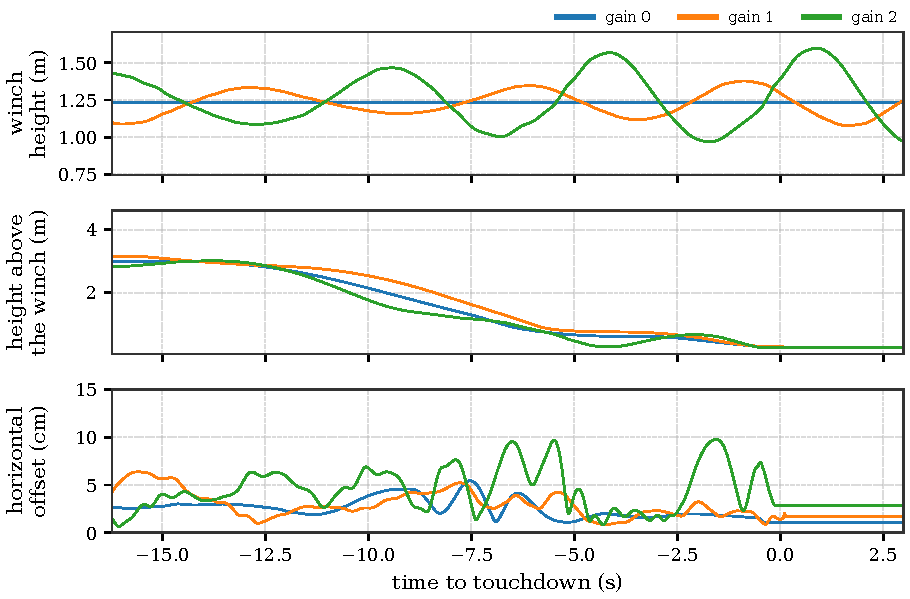
\includegraphics[width=\textwidth]{Results/figures/03_disturbances/waves_landing.pdf}
    \caption[Landing with waves.]{Landing with waves, from the start of the descent to the touchdown: height of the winch, height of the \gls{uav} above it, and horizontal offset of the \gls{uav} from it.}
    \label{fig:res_waves}
\end{figure}

% Does the UAV stay above the pad while the deck moves?
The landing is not affected by the heave in its timing. It takes between $25$ and $27\,\text{s}$ for the three sea states, and the \gls{uav} descends in the same way, since its reference is taken above the mean height of the winch and does not follow the deck up and down. The horizontal offset from the winch stays within $5\,\text{cm}$ during the descent on a calm sea and with a gain of $1$, and within $10\,\text{cm}$ with a gain of $2$, as the deck rolls under the \gls{uav}. The touchdown is $0$, $2$ and $4\,\text{cm}$ from the centre of the pad.

% What does the heave change, then?
What the heave changes is the contact. The final approach aims at a point below the deck, so that the \gls{uav} touches down even if the deck falls away from it. The speed of the contact is then set by the motion of the deck, and grows with the waves, from $0.15\,\text{m/s}$ on a calm sea to $0.26$ and $0.39\,\text{m/s}$ with gains of $1$ and $2$. In every case, the winch then holds the \gls{uav} against the pad, and it remains there as the deck keeps moving.

\subsection{Wind}
\label{subsec:res_wind}
% Increasing wind, with and without the disturbance estimate
